\documentclass{article}
%\renewcommand{\rmdefault}{ppl}
%\usepackage{personal}
\usepackage{graphicx}
\usepackage{placeins}

\usepackage{amsmath}
\usepackage{wasysym}
\usepackage{amssymb}

\usepackage{array}
\newcolumntype{L}[1]{>{\raggedright\let\newline\\\arraybackslash\hspace{0pt}}m{#1}}
\newcolumntype{C}[1]{>{\centering\let\newline\\\arraybackslash\hspace{0pt}}m{#1}}
\newcolumntype{R}[1]{>{\raggedleft\let\newline\\\arraybackslash\hspace{0pt}}m{#1}}
\usepackage{booktabs}
\usepackage{tabularx}
%\usepackage[font=small]{caption}
%\usepackage[strings]{underscore}
%\usepackage{subfigure}
\usepackage{color}
\usepackage{floatflt}
\usepackage[table]{xcolor}
\definecolor{Gray}{gray}{0.9}
%\usepackage[boxed]{algorithm2e}
%\usepackage{lmacro}
%\topmargin=-0.5in\usepackage[table]{xcolor}
\definecolor{White}{rgb}{1,1,1}
\definecolor{Gray}{gray}{0.9}
\definecolor{LightCyan}{rgb}{0.88,1,1}
\usepackage{soul}
\usepackage{sidecap}
\graphicspath{{./Figures/}}
%\usepackage[margin=1.2in]{geometry}
\usepackage{hyperref}
\hypersetup{colorlinks=true,
citecolor=blue,
linkcolor=black,
urlcolor=black}

\usepackage{algorithm,algorithmicx}
\usepackage[noend]{algpseudocode}
\newcommand*\DNA{\textsc{dna}}

\newcommand*\Let[2]{\State #1 $\gets$ #2}
\algrenewcommand\algorithmicrequire{\textbf{Precondition:}}
\algrenewcommand\algorithmicensure{\textbf{Postcondition:}}
%\usepackage{fontspec}
%\setmainfont{Hoefler Text}
%\newcommand*\DNA{\textsc{dna}}
%
%\newcommand*\Let[2]{\State #1 $\gets$ #2}
%\algrenewcommand\alglinenumber[1]{
%    {\sf\footnotesize\addfontfeatures{Colour=888888,Numbers=Monospaced}#1}}
%\algrenewcommand\algorithmicrequire{\textbf{Precondition:}}
%\algrenewcommand\algorithmicensure{\textbf{Postcondition:}}

\title{{\bf \huge $\epsilon$}-Lexicase selection: a probabilistic and multi-objective analysis of lexicase selection and with continuous valued problems}
\author{William La Cava, Lee Spector, Jason Moore}

\date{December 2016}


\begin{document}

%\numberofauthors{3}
%
%\alignauthor
%William La Cava\titlenote{corresponding author} \\
%       \affaddr{Department of Mechanical and Industrial Engineering}\\
%       \affaddr{University of Massachusetts}\\
%       \affaddr{Amherst, MA 01003}\\
%       \email{wlacava@umass.edu}
%%%\alignauthor
%%%Thomas Helmuth\\
%%%       \affaddr{Department of Computer Science}\\
%%%       \affaddr{University of Massachusetts}\\
%%%       \affaddr{Amherst, MA 01003}\\
%%%       \email{thelmuth@umass.edu}
%\alignauthor
%Lee Spector\\
%       \affaddr{School of Cognitive Science}\\
%       \affaddr{Hampshire College}\\
%       \affaddr{Amherst, MA 01002}\\
%       \email{lspector@hampshire.edu}
%\and
%\alignauthor
%Kourosh Danai\\
%       \affaddr{Department of Mechanical and Industrial Engineering}\\
%       \affaddr{University of Massachusetts}\\
%       \affaddr{Amherst, MA 01003}\\
%       \email{danai@engin.umass.edu}
%}

%\maketitle
%\ead{danai@ecs.umass.edu}
%\cortext[cor1]{Corresponding author}
%\address[mie]{D, , Amherst, MA 01003}
%\address[hc]{School of Cognitive Science, Hampshire College, Amherst MA 01002}
%

\maketitle
\begin{abstract}
Lexicase selection is a parent selection method that considers test cases separately, rather than in aggregate, when performing parent selection. As opposed to previous work that has demonstrated the ability of lexicase selection to solve difficult problems, the goal of this paper is to develop the theoretical underpinnings that explain its performance. To this end, we derive an analytical formula that gives the expected probabilities of selection under lexicase selection, given a population and its behavior. In addition, we expand upon the relation of lexicase selection to many-objective optimization methods to show the effect of lexicase, which is to select individuals on the boundaries of Pareto fronts in high-dimensional space. We show analytically why lexicase selection performs more poorly for certain sizes of population and training cases, and why it has been shown to perform more poorly in continuous error spaces. To addres this last concern, we introduce $\epsilon$-lexicase selection, which modifies the pass condition defined in lexicase selection to allow near-elite individuals to pass cases, thereby improving selection performance. We show that $\epsilon$-lexicase outperforms several diversity-maintenance strategies for regression problems.
\end{abstract}


\section{INTRODUCTION}
  

\section{Lexicase Selection}\label{s:2}
Lexicase selection is a parent selection technique based on lexicographic ordering of test (i.e. fitness) cases.  Each parent selection event proceeds as follows: 

\begin{enumerate}
\item The entire population is added to the selection pool.
\item The fitness cases are shuffled.
\item Individuals in the pool with a fitness worse than the best fitness on this case among the pool are removed. 
\item If more than one individual remains in the pool, the first case is removed and 3 is repeated with the next case. If only one individual remains, it is the chosen parent. If no more fitness cases are left, a parent is chosen randomly from the remaining individuals. 
\end{enumerate}

The lexicase selection algorithm for a single selection event is presented below: 
\noindent{\footnotesize
\begin{tabularx}{\textwidth}{lX}
\multicolumn{2}{c}{\textbf{Lexicase Selection}} \\ 
\texttt{GetLexicaseParent}($\mathcal{N,T}$) 	:						&	\\
\hspace{1em}	$T' \leftarrow \texttt{shuffle(}\mathcal{T})$	&	training cases\\
\hspace{1em}	$S \leftarrow \mathcal{N}$	&	initial selection pool is the population\\
\hspace{1em}	while $|T'| >0$ and $|\mathcal{S}|>1$:						&	main loop\\
\hspace{1em}\hspace{1em}	\texttt{case} $\leftarrow$ random choice from $\mathcal{T'}$ 	&	choose a random case\\
\hspace{1em}\hspace{1em}	\texttt{elite} $\leftarrow$ best fitness in $\mathcal{S}$ on \texttt{case} 	&	determine elite fitness\\
\hspace{1em}\hspace{1em}	$\mathcal{S} \leftarrow n \in \mathcal{S}$ if fitness($n$) = \texttt{elite}				&	reduce selection pool to elites\\
\hspace{1em}\hspace{1em}	$\mathcal{T'} \leftarrow \mathcal{T'} - $ \texttt{case}				&	remove top case\\
\hspace{1em} return random choice from $\mathcal{S}$															&	return parent  
\end{tabularx}
}
%\begin{algorithm}
%  \caption{Lexicase Selection}\label{alg:lexicase}
%  \begin{algorithmic}[1]
%    \Statex
%    \Function{GetParent}{$\mathcal{N}, \mathcal{T}$}
%    	\Let{$T'$}{shuffle($\mathcal{T}$)} \Comment{Shuffle the test cases}	
%    	\Let{$N'$}{$\mathcal{N}$}
%    	\Let{$parent$}{$\emptyset$}
%		\While{$|T'| > 0$ and $|N'|>1$}
%      		\Let{\texttt{case}}{$T'[0]$}
%      		\Let{\texttt{best\_fit}}{$\infty$}
%        	\For{$n \in N'$}
%        		\If{fitness of $n$ on \texttt{case} $<$ \texttt{best\_fit}}
%          			\Let{\texttt{best\_fit}}{fitness of $n$ on \texttt{case}}
%          			\Let{$parent$}{$n$}
%          		\ElsIf{fitness of $n$ on \text{case} $=$ \texttt{best\_fit}}	
%          			\Let{$parent$}{$parent \cup n$}
%        		\EndIf
%			\EndFor
%        	\Let{$T'$}{$T'-$\texttt{case}}
%        	\Let{$N'$}{$parent$}
%		\EndWhile
%	\State \Return{random choice from $parent$}
%    \EndFunction
%  \end{algorithmic}
%\end{algorithm}
\section{{\large $\epsilon$}-Lexicase Selection}\label{s:2}

\noindent{\footnotesize
\begin{tabularx}{\textwidth}{lX}
\multicolumn{2}{c}{\textbf{$\epsilon$-Lexicase Selection}} \\ 
\texttt{Get\_$\epsilon$-Lexicase\_Parent}($\mathcal{N,T}$) 	:						&	\\
\hspace{1em}	$T' \leftarrow \texttt{shuffle(}\mathcal{T})$	&	training cases\\
\hspace{1em}	$S \leftarrow \mathcal{N}$	&	initial selection pool is the population\\
\hspace{1em}	$\epsilon \leftarrow MAD$(fitness($\mathcal{N}$)) for $t \in \mathcal{T}$	&	get $\epsilon$ for each case\\
\hspace{1em}	while $|T'| >0$ and $|\mathcal{S}|>1$:						&	main loop\\
\hspace{1em}\hspace{1em}	\texttt{case} $\leftarrow T'[0]$ 	&	consider the top case\\
\hspace{1em}\hspace{1em}	\texttt{elite} $\leftarrow$ best fitness in $\mathcal{S}$ on \texttt{case} 	&	determine elite fitness\\
\hspace{1em}\hspace{1em}	$\mathcal{S} \leftarrow n \in \mathcal{S}$ if fitness($n$) $<=$ \texttt{elite}$+\epsilon_{\texttt{case}}$	&	reduce selection pool to elites\\
\hspace{1em}\hspace{1em}	$\mathcal{T'} \leftarrow \mathcal{T'} - $ \texttt{case}				&	remove top case\\
\hspace{1em} return random choice from $\mathcal{S}$															&	return parent  
\end{tabularx}
}
%\begin{algorithm}
%  \caption{$\epsilon$-Lexicase Selection}\label{alg:lexicase}
%  \begin{algorithmic}[1]
%    \Statex
%    \Function{GetParent}{$\mathcal{N}, \mathcal{T}$}
%    	\Let{$T'$}{shuffle($\mathcal{T}$)} \Comment{Shuffle the test cases}	
%    	\Let{$N'$}{$\mathcal{N}$}
%    	\Let{$parent$}{$\emptyset$}
%    	\For{$t \in \mathcal{T}$}
%    		\Let{$M\{t\}$}{$MAD(t,N')$}
%    	\EndFor
%		\While{$|T'| > 0$ and $|N'|>1$}
%      		\Let{\texttt{case}}{$T'[0]$}
%      		\Let{\texttt{best\_fit}}{$\infty$}
%        	\For{$n \in N'$}
%        		\If{fitness of $n$ on \texttt{case} $<$ \texttt{best\_fit}}
%          			\Let{\texttt{best\_fit}}{fitness of $n$ on \texttt{case}}
%          		\EndIf
%          	\EndFor
%          	\For{$n \in N'$}		
%          		\If{fitness of $n$ on \texttt{case} $<$ \texttt{best\_fit} + $M\{case\}$}
%          			\Let{$parent$}{$parent \cup n$}
%        		\EndIf
%			\EndFor
%        	\Let{$T'$}{$T'-$\texttt{case}}
%        	\Let{$N'$}{$parent$}
%		\EndWhile
%	\State \Return{random choice from $parent$}
%    \EndFunction
%  \end{algorithmic}
%\end{algorithm}


\begin{table}

\end{table}
\subsection{Expected Probabilities of Selection}
What is the probability of an individual being selected, given its performance in a given population on a set of training cases?  

\noindent $\mathcal{N} = \{n_i\}_{i=1}^N$: population \\
$\mathcal{T} = \{t_i\}_{i=1}^T$: training cases\\
$\mathcal{K}_n = \{k_i\}_{i=1}^K \subseteq \mathcal{T}$: training cases from $\mathcal{T}$ for which individual $n$ is elite\\


To put it in words, the probability of $n$ being selected is the probability that a case $n$ passes ($t \in \mathcal{K}_n$) is selected and: \begin{enumerate} \item no more cases remain and $n$ is selected among the set of individuals that pass the selected case; or \item $n$ is the only individual that passes the case; or \item $n$ is selected via the selection of another case that $n$ passes (repeating the process). \end{enumerate} 

Formally, let $P_{sel}(n | \mathcal{N}, \mathcal{T}, \mathcal{K}_n)$ be the probability of $n$ being selected in a population $\mathcal{N}$ with training cases $\mathcal{T}$. Let $\mathcal{K}_n(\mathcal{T})$ be the subset of cases in $\mathcal{T}$ for which $n$ is elite. Then lexicase probability can be represented as a piecewise recursive function: 


{\scriptsize
\begin{align}\label{eq:prob}
P_{sel}(n | \mathcal{N}, \mathcal{T}) &= \\
 &\left\{\nonumber 
     \begin{array}{lcr}
       1 & : & |\mathcal{T}| >0, |\mathcal{N}| = 1; \\
       1/|\mathcal{N}| & : &|\mathcal{T}| = 0; \\ 
       \frac{1}{|\mathcal{T}|}\sum_{k_s \in K_n(\mathcal{T})}{P_{sel} \left( n | \mathcal{N}(m|k_s \in K_m(\mathcal{T})), \mathcal{T}(t|t \neq k_s) \right)} & : & \text{otherwise}
     \end{array}
   \right. 
\end{align}
}

The first two elements of $P_{sel}$ follow from the lexicase algorithm: if there is one individual in $\mathcal{N}$, then it is selected; if there no more cases in in $\mathcal{T}$, then $n$ has a probability of selection split among the individuals in $\mathcal{N}$, i.e.,  $1/|\mathcal{N}|$. If neither of these conditions are met, the remaining probability of selection is $1/|\mathcal{T}|$ times the summation of $P_{sel}$ over $n$'s elite cases. Each case for which $n$ is elite (represented by $k_s \in K_n(\mathcal{T})$) has a probability of $1/|\mathcal{T}|$ of being selected. For each potential selection $k_s$, the probability of $n$ being selected as a result of this case being chosen is dependent on the number of individuals that are also elite on these cases, represented by $\mathcal{N}(m|k_s \in K_m(\mathcal{T}))$, and the cases that are left to be chosen, represented by $\mathcal{T}(t|t \neq k_s) )$. 

\paragraph{Example}
As an example of calculating absolute probabilities, we consider the illustrative problem from the original lexicase selection paper~\cite{spector_assessment_2013}, shown in Table~\ref{tbl:ex}. Using Eqn.~\ref{eq:prob}, the probabilities for each individual can be calculated as follows:

\begin{align*}
P_{sel}(n_1) &=& 1/4*(1/3*(1)+1/3*(1+1)) = 0.25 \\
P_{sel}(n_2) &=& 1/4*(0) = 0 \\
P_{sel}(n_3) &=&1/4*(1/3*(1+1/2*(1))+1/3*(1)) = 0.20833 \\
P_{sel}(n_4) &=& 1/4*(1/3*(1/2*(1)+1)+1/3*(1)) = 0.20833 
\end{align*}

\begin{table}
\centering
\caption{Example population from original lexicase paper (Spector 2013).}\label{tbl:ex}
\begin{tabular}{l|cccc|c|r|rr}
Program & \multicolumn{4}{c}{Test} & $\mathcal{K}(\mathcal{T})$ & MAE & $P_{sel}$ & $P_{t}$\\
& $t_1$ & $t_2$ & $t_3$ & $t_4$ & \\ \hline
$n_1$ & 2 & 2 & 4 & 2 & $\{t_2,t_4\}$ &	2.5		&	0.25 	& 	0.28	\\
$n_2$ & 1 & 2 & 4 & 3 & $\{t_2\}$		&	2.5		&	0.00	&	0.28	\\
$n_3$ & 2 & 2 & 3 & 4 & $\{t_2,t_3\}$ &	2.75	& 	0.33	&	0.12	\\
$n_4$ & 0 & 2 & 5 & 5 & $\{t_1,t_2\}$ &	3.0		& 	0.208	&	0.04	\\
$n_5$ & 0 & 3 & 5 & 2 & $\{t_1,t_4\}$ &	2.5		&	0.208	&	0.28
\end{tabular}
\end{table}

We compare the probability of selection under lexicase selection to that using tournament selection with an indentical population and fitness structure. To do so we must first formulate the probability of selection for an individual undergoing tournament selection with $r$-size tournaments. Consider that the mean absolute error is used to aggregate the fitness cases. Then the fitness ranks of $\mathcal{N}$ can be calculated, with lower rank indicating better fitness. Let $S_i$ be the individuals in $\mathcal{N}$ with a fitness rank of $i$, and let $Q$ be the number of unique fitness ranks. Then Xie et. al. (cite) showed that the probability of selecting an individual with rank $j$ in a single tournament is 
\begin{equation}
P_t = \frac{1}{|S_j|}\left( \left(\frac{\sum_{i=j}^Q{|S_i|}}{N}\right)^r - \left(\frac{\sum_{i=j+1}^Q{|S_i|}}{N}\right)^r \right)
\end{equation}



\begin{figure}
\centering
  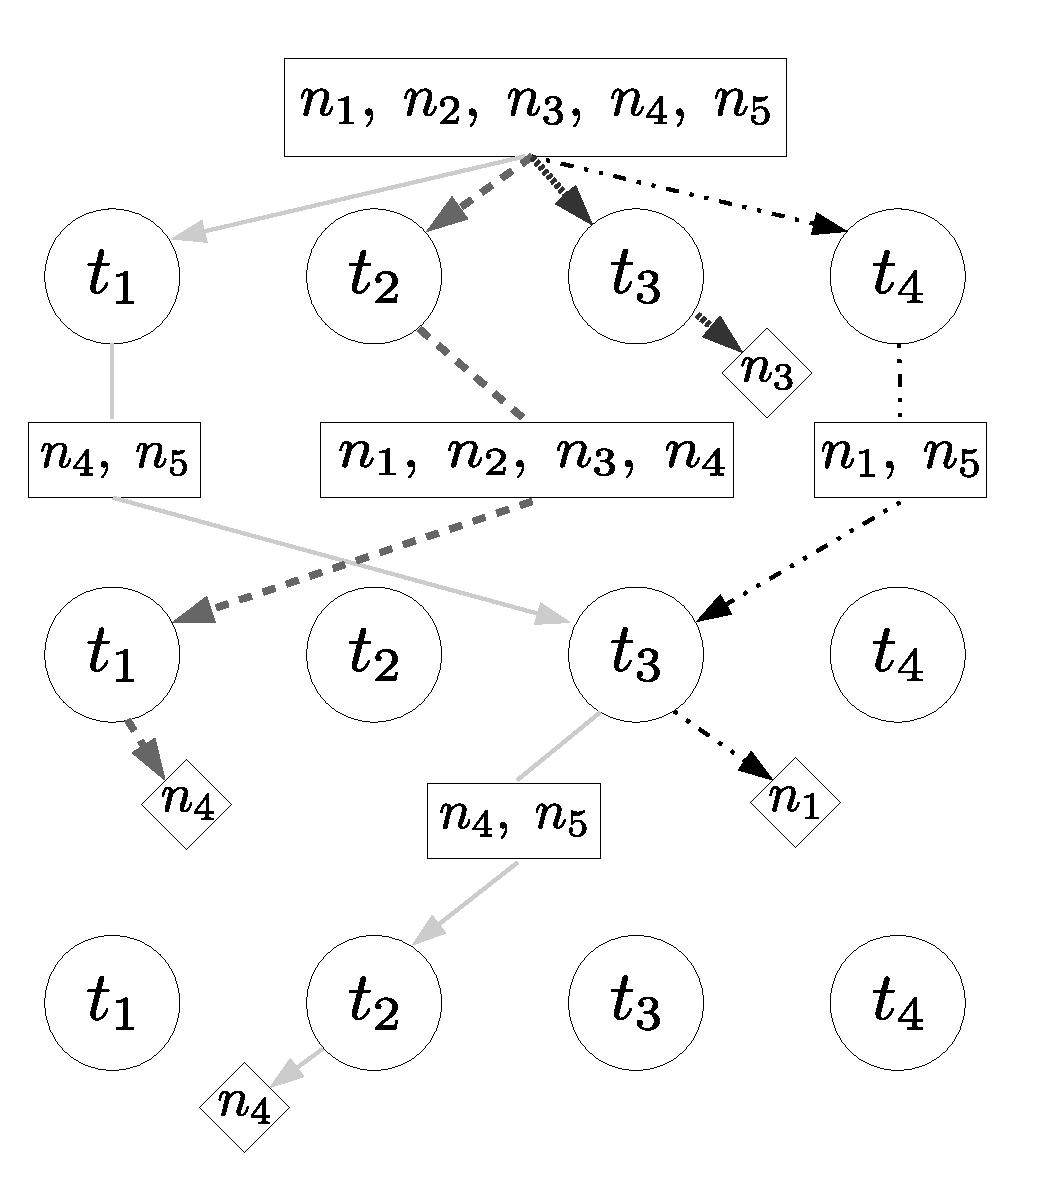
\includegraphics[height = 0.4\textheight]{figs/lex_graph.pdf}\\
  \caption{A graphical representation of 3 example parent selections using lexicase selection on the population in Table~\ref{tbl:ex}. The bold, dashed and dot-dashed lines indicate different selection paths through the test cases in circles. The boxes indicate the selection pool at each step in the process.}\label{fig:boxplot_eps_e}
\end{figure}

\paragraph{Complexity}
Can we analytically calculate the probability of selection an individual with less complexity than executing the lexicase selection algorithm? It appears not. Eqn.~\ref{eq:prob} has a worst-case complexity of $O(T^N)$ when all individuals are elite on $\mathcal{T}$, which discourages its use as a selection method. The lexicase selection algorithm samples the expected probabilities of each individual by recursing on random orders of cases in $\mathcal{T}$, considering one at a time rather than branching to consider all combinations of cases that could result in selection for each individual in question. This gives lexicase selection a complexity of $O(TN)$ for selecting a single parent, and therefore a complexity of $O(TN^2)$ per generation. 


 
\subsection{Effect of $N$ and $T$}
What does the an analysis of the probability of selection for lexicase selection tell us about how lexicase behaves for cases in which $|\mathcal{N}| << |\mathcal{T}|$?   $|\mathcal{T}| << |\mathcal{N}|$ ? 

The sampling of $P_{sel}$ done by lexicase is tied to the population size because lexicase selection conducts $N$ depth-first searches of the case orderings to choose $N$ parents. This implies that the value of $N$ determines the fidelity with which $P_{sel}$ is approximated via the sampling. Smaller populations will therefore produce poorer approximations of $P_{sel}$. 

The effectiveness of lexicase selection has also been tied to the number of fitness cases, $T$. When $T$ is small, there are very few ways in which individuals can be selected. For example, if $T$ = 2, an individual must be elite on one of these two cases to be selected. For continuous errors in which few individuals are elite, this means that only two individuals are likely to produce all of the children for the subsequent generation.

\subsection{Effect of different population structures}

\begin{enumerate}
\item compare probability of lexicase selection to probability of selection with tournament / roulette 
\item compare population structures: maintain correlation structure and vary population size/ number of test cases
\item see how many iterations of lexicase selection are required to converge on the probabilities of selection for the example problem in Table~\ref{tbl:ex}
\item population where there is one individual that sucks at everything but is good at other things - how does it compare to tournament selection probabilities?
\item do not assume that $N$ rounds of lexicase selection are conducted!
\end{enumerate}

\section{Multi-objective Interpretation of Lexicase Selection}
Lexicase selection is guarantees the return of individuals that are on the Pareto front with respect to the fitness cases. This is a necessary but not sufficient condition. In fact, lexicase selection only selects those individuals in the ``corners" of the Pareto front, meaning they are on the front {\it and} elite, globally, with respect to at least one fitness case. Put another way, no individual can be selected via lexicase selection unless it is elite with respect to at least one objective among the entire population, regardless of its performance on other objectives. 

Interestingly, the worst-case complexity of NSGA-II is the best-case complexity for lexicase selection. Add notes from discourse

Farina and Amato~\cite{farina_optimal_2002}: \begin{quote}
the Pareto definition of optimality in a multi-criteria decision making problem can be unsastisfactory due to essentially two reasons: the number of improved or equal objective values is not taken into account, the (normalized) size of improvements is not taken into account
\end{quote}
\begin{figure}
\centering
  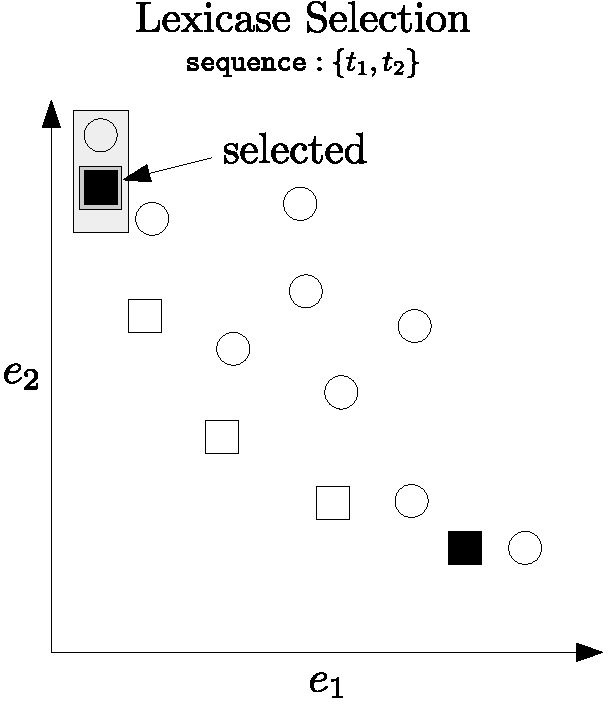
\includegraphics[width = \textwidth]{figs/lex_pareto.pdf}\\
  \caption{An illstration of the performance of lexicase selection and $\epsilon$-lexicase selection in a scenario involving two cases. Each point represents and individual in the population. The squares are individuals on the Pareto front. In each case, the selection ordering shown is $\{t_1,t_2\}$. }\label{fig:boxplot_eps_e}
\end{figure}
%Here is a detailed look at selection for program $n_1$:
%\begin{align*}
%P_{sel}(n_1 | \mathcal{N}, \mathcal{T}) &= \frac{1}{|\{t_1,t_2,t_3,t_4\}|}  \sum_{k_s \in \{t_2,t_4\}}{ P_{sel} \left( n_1 | \mathcal{N}(m|k_s \in K_m(\mathcal{T})), \mathcal{T}(t|t \neq k_s) \right)}  \\
%&= \frac{1}{4} \biggl[ P_{sel} \left( n_1 | \mathcal{N}(m|t_2 \in K_m(\mathcal{T})), \mathcal{T}(t|t \neq t_2) \right) + P_{sel} \left( n | \mathcal{N}(m|t_4 \in K_m(\mathcal{T})), \mathcal{T}(t|t \neq t_4) \right) \biggl] \\
%&= \frac{1}{4} \left[ P_{sel} ( n | \{n_1, n_2, n_3, n_4\}, \{t_1, t_3, t_4\} ) + P_{sel} ( n | \{n_1, n_5 \} , \{t_1, t_2, t_3\} ) \biggl] \\
%&= \frac{1}{4} \biggl[ \frac{1}{|\{t_1, t_3, t_4\}} \sum_{k_s \in \{t_4\}}{ P_{sel} \left( n | \mathcal{N}(m|k_s \in K_m(\mathcal{T}(t|t \neq t_2)), \mathcal{T}(t|t \notin \{t_2,k_s\}) \right)} \\
%& + \frac{1}{|\{t_1, t_2, t_3\}|} \sum_{k_s \in \{t_2,t_3\}}{ P_{sel} \left( n | \mathcal{N}(m|k_s \in K_m(\mathcal{T}(t|t \neq t_2)), \mathcal{T}(t|t \notin \{t_4,k_s\}) \right)}\biggl] \\
%&= \frac{1}{4} \biggl[ \frac{1}{3} P_{sel} ( n_1 | \{n_1\}, \{t_1, t_3\})  + \frac{1}{3} \biggl( P_{sel} ( n_1 | \{n_1\}, \{t_1,t_3\} ) \\
%&+ P_{sel} ( n_1 | \{n_1\}, \{t_1,t_2\} ) \biggl) \biggl]\\
%&= \frac{1}{4} \biggl[ \frac{1}{3}(1) + \frac{1}{3}(1 + 1) \biggl]\\
%&= \frac{1}{4} 
%\end{align*}
Here we define Pareto dominance relations with respect to the training cases. 

\medskip
\noindent {\bf Definition:} $n_1$ dominates $n_2$, i.e., ${n_1} \prec {n_2}$, if $e_j(n_1) \leq e_j(n_2) \;
\forall j  \in \{1,\dots,N\}$ and $\exists j \in \{1,\dots,N\}$ for which $e_j(n_1) < e_j(n_2)$. \bigskip
\bigskip

\medskip
\noindent \textbf{Theorem 1:} Individuals selected by lexicase selection are non-dominated in $\mathcal{N}$ with respect to the training cases $\mathcal{T}$. 
\medskip

\noindent \textbf{Proof:} Let $n_1, n_2 \in \mathcal{N}$ be individuals in a population selected by lexicase selection. Suppose $n_1 \prec n_2$. Then $e_j(n_1) \leq e_j(n_2) \;
\forall j  \in \{1,\dots,N\}$ and $\exists j \in \{1,\dots,N\}$ for which $e_j(n_1) < e_j(n_2)$. Therefore $n_1$ is selected for every case that $n_2$ is selected, and $\exists t \in \mathcal{T}$ for which $n_2$ is removed from selection due to $n_1$. Therefore $n_2$ cannot be selected by lexicase selection, the supposition is false, and the theorem is true. 
\bigskip


We can extend Theorem 1 to $\epsilon$-lexicase selection for conditions in which $\epsilon$ is pre-defined for each fitness case, i.e. in static and dynamic cases, but not when $\epsilon$ is recalculated for each selection pool. The theorem is extended by defining the dominance relation with respect to $\epsilon$, as follows:


\medskip
\noindent {\bf Definition:} $n_1$ $\epsilon$-dominates $n_2$, i.e., ${n_1} + \epsilon_j \prec_{\epsilon} {n_2}$, if $e_j(n_1) \leq e_j(n_2)  \;
\forall j  \in \{1,\dots,N\}$ and $\exists j \in \{1,\dots,N\}$ for which $e_j(n_1) + \epsilon_j < e_j(n_2) $. \bigskip
\bigskip

In this case, the analagous condition holds for individuals selected with $\epsilon$-lexicase selection. 

\medskip
\noindent \textbf{Theorem 2:} Individuals selected by $\epsilon$-lexicase selection are non-$\epsilon$-dominated in $\mathcal{N}$ with respect to the training cases $\mathcal{T}$. 
\medskip


\noindent \textbf{Proof:} Let $n_1, n_2 \in \mathcal{N}$ be individuals in a population selected by $\epsilon$-lexicase selection. Suppose $n_1 \prec_{\epsilon} n_2$. Then $e_j(n_1) \leq e_j(n_2) + \epsilon_j\;
\forall j  \in \{1,\dots,N\}$ and $\exists j \in \{1,\dots,N\}$ for which $e_j(n_1) < e_j(n_2) + \epsilon_j$. Therefore $n_1$ is selected for every case that $n_2$ is selected, and $\exists t \in \mathcal{T}$ for which $n_2$ is removed from selection due to $n_1$. Therefore $n_2$ cannot be selected by lexicase selection, the supposition is false, and the theorem is true. 
\bigskip


\section{Related Work}\label{s:3}


\section{Experimental Analysis} \label{s:4}

\begin{table}
\scriptsize
\caption{Symbolic regression problem settings.}\label{tbl:symreg_settings}
\begin{tabularx}{\columnwidth}{X R{0.57\columnwidth}} \toprule
Setting& Value \\ \midrule
Population size & 1000 \\
Crossover / mutation & 80/20\% \\
Program length limits & [3, 50] \\ 
ERC range & [-1,1] \\
Generation limit & 1000 \\
Trials & 30 \\
Terminal Set & \{$\mathbf{x}$, ERC, $+$, $-$, $*$, $/$, $\sin$, $\cos$, $\exp$, $\log$\}\\
Elitism & keep best \\
\end{tabularx}
\end{table}
\begin{table}
\scriptsize
\caption{Problems used for method comparisons.}\label{tbl:datasets}
\begin{tabularx}{\columnwidth}{X r r r} \toprule
\multicolumn{4}{c}{Regression}\\ 
Problem & Dimension & Training Cases & Test Cases \\ \midrule
Housing & 14 & 354 & 152 \\
Tower & 25 & 2195 &  940 \\
Wind & 6 & 4200 & 1800 \\
ENH & 8 & 538 & 230 \\
ENC & 8 & 538 & 230 \\
UBall5D & 5 & 1024 & 5000 \\ \midrule
\end{tabularx}
\begin{tabularx}{\columnwidth}{X X r r r} 
\multicolumn{5}{c}{Dynamical Systems}\\ \midrule
Problem & Equations & Initial Conditions	& Training Cases & Test Cases \\ \midrule
\end{tabularx}
\begin{tabularx}{\columnwidth}{X X r r r} 
\multicolumn{5}{c}{Program Synthesis}\\ 
Problem	& Input & Output	& Training Cases & Test Cases \\\midrule
Number IO & integer in [-100,100], float in [-100.0, 100.0]	&	printed float & 25 & 1000 \\
Wallis PI & integer in [1, 200] & float &	150 & 50 \\
Vector Average & vector of float of length [1,50] with each float in [-1000.0, 1000.0]	& float &	100	&	1000 \\ 
\bottomrule
\end{tabularx}

\end{table} 


\subsection{Effect of population structure on probabilities of selection}


\subsection{Results}\label{s:4 results}

\section{Discussion}\label{s:5}


\section{Conclusions}\label{s:6}

\section{Acknowledgments}
The authors would like to thank Thomas Helmuth, Nic McPhee and Bill Tozier for their feedback as well as members of the Computational Intelligence Laboratory at Hampshire College. This work is partially supported by NSF Grant Nos. 1068864, 1129139 and 1331283. Any opinions, findings, and conclusions or recommendations expressed in this publication are those of the authors and do not necessarily reflect the views of the National Science Foundation. This work used the Extreme Science and Engineering Discovery Environment (XSEDE), which is supported by NSF grant number ACI-1053575~\cite{towns_xsede:_2014}.


\bibliographystyle{abbrv}
\bibliography{epsilon_lexicase}


\end{document}
